\chapter{Technology Used}\label{chap:tech}

\section{Go Programming Language}

We chose the Go Programming Language because it has a built-in concurrency model that will allow 
us to scale the architecture in the future and prepare it for real-world usage. 
The language implements this model directly with the \emph{goroutine}. Additionally,
using the Go module made it easy to share code between different modules 
without spending too much time on the design of a general solution. 
This choice also enabled us to implement the analysis feature described in Section \ref{sec:lnmetrics_server} 
by importing one module from the analysis system into the plugin described in Section \ref{sec:lnmetrics_client}.

\section{{\CLN} Plugin API}

The most difficult part of prototyping the implementation of lnmetrics on a real 
lightning implementation was dealing with the differences between the implementations, 
as they all have different APIs. For the initial prototyping described in this document,
we work with {\CLN} by using the {\CLN} Plugin API, which allows 
anyone to extend the API of {\CLN} with a plugin written in any language and then
extend the design to support other lightning implementations.
The Core Lightning plugin API enables the registration 
of a new \emph{JSON RPC 2.0}\cite{jsonrpc} method and listening to 
events generated by the node through JSON RPC 2.0 notifications.

\subsection{GO API library for {\CLN}}
\label{sec:go-api}
To interact with the core lightning node, we chose to implement a Go API for core 
lightning, which is available on Github at \url{https://github.com/vincenzopalazzo/cln4go}. 
This library has not been updated to the current version of the core lightning 
API and it has been written with an older version of Go that did not support generics. 
The generics feature implemented in Go language 1.18 allows for writing 
strongly-typed libraries and defining the type inside the user module instead of the library. 
This approach supports all core lightning versions and allows users to choose 
which version to support at the application level.

We designed the API library in this way because the core lightning API is 
evolving quickly, and sometimes the node is not using the most recent version. 
Users may be one or two versions behind; hence our solution allows the author of 
the plugin to enforce any rules regarding the core lightning version without being 
constrained by the developer of the core lightning plugin API.

Additionally, the library allows the specification of the JSON encoder to use 
at runtime, enabling the use of more performant libraries 
such as \emph{go-json}\cite{gojson}. This feature is 
important for removing some of the pain points of the Go language, 
such as the reflection used during the encoding and decoding of JSON from and 
to a Go struct. We measured the performance of our library against the well-known 
glightning library \cite{glightning}, and the results are shown 
in Figure \ref{fig:api-go-bench}.

\begin{figure}[H]
    \begin{center}
      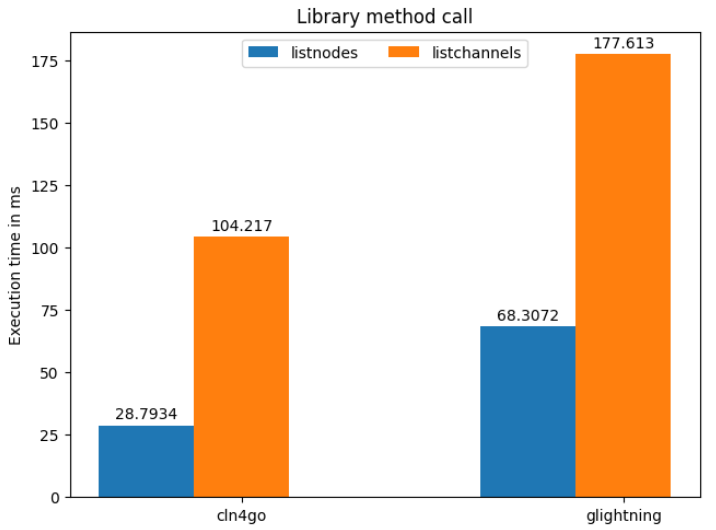
\includegraphics[scale=0.5]{imgs/api-go-bench.png}
    \end{center}
    \caption{Comparison between networks of the Lightning Node size.}
    \label{fig:api-go-bench}
\end{figure}

This figure shows two Core Lightning Method calls: listnodes and listchannels. listnodes
returns all the nodes on the Lightning Network that the node can see from the
gossip map, while listchannels returns the complete list of channels that are announced
on the network, and the benchmarks show that the library that we are proposing is faster
than the popular library glightning.


\section{lnmetrics.utils}

To implement the entire architecture in Go Language, we needed to write shared 
code to be used in all of our projects, such as database code and a logger. 
To provide this shared code in one place and to implement missing features 
around the Go ecosystem, such as a powerful time library that allows for 
operations on the Unix timestamp, we developed a library called lnmetrics.utils. 
This library contains all the code that we share across our projects and is 
available on Github at \url{https://github.com/LNOpenMetrics/lnmetrics.utils}.

\section{GraphQL and GQLGen}

\subsection{GraphQL Protocol}

To implement an analysis system with a public API, as  described in 
Section \ref{sec:lnmetrics_server}, we chose to use the GraphQL protocol \cite{graphql}. 
This protocol implements a query language and runtime for APIs that was 
developed by Facebook in 2012 and released as an open-source project in 2015. 
GraphQL is designed to enable clients to specify exactly what data they need 
from an API, and nothing more. This is achieved through a typed schema that 
describes the data available in the API and a set of queries that clients can 
use to request the specific data they need. Unlike REST APIs, which often require 
multiple requests to fetch related data, GraphQL allows clients to retrieve all 
the necessary data in a single request. This makes it particularly useful for 
mobile and web applications where minimizing the number of network 
requests can improve performance.

\subsection{GQLGen Library}

In order to implement the GraphQL protocol \cite{graphql} in the analysis system, we used the library
gqlgen \cite{gqlgen}, which is a Go library for building GraphQL servers that follow the GraphQL specification. 
It generates Go code from a GraphQL schema and a set of resolver functions, which the developer writes
to handle the queries and mutations defined in the schema. The generated code 
provides a strongly typed API that can be used to interact with the GraphQL server.

One of the benefits of using gqlgen is that it allows for a clear separation of 
concerns between the schema definition and the resolver implementation. This makes it 
easier to maintain and evolve the schema over time, without having to modify the resolver code.

\section{JSON Schema}

In order to define a description of the data model described in Section \ref{sec:data_definition}
we use JSON Schema. JSON Schema is an important, evolving standard schema language for families of JSON documents, and it is based on a complex combination of structural operators, Boo\-le\-an operators, including full negation,  and mutually recursive variables. JSON Schema is particularly useful for defining APIs that exchange data in JSON 
format; indeed, by defining a schema for the data, clients can know exactly what data 
they can expect to receive from the API and how it should be structured.
A schema is defined using JSON itself and consists of a set of keywords 
that describe constraints on the  format and the structure of the data. 
Overall, JSON Schema provides a powerful and flexible way to define the structure of 
JSON data and is an important tool for building APIs that exchange data in JSON format.
